\subsubsection{Behavioral Cloning}
\label{sec:bc}
\begin{algorithm}[t]
\caption{Abstract Algorithm for BC methods}\label{alg:bc}
\begin{algorithmic}
\REQUIRE A set of expert demonstrations $\mathcal{D}^{E}$, a parameterized policy $\pi_{\theta}^{L}$
\ENSURE The optimal set of policy parameter $\theta^{*}$
\STATE Optimize $\mathcal{L}$ w.r.t.\ policy parameter $\theta$ using $\mathcal{D}^{E}$
\end{algorithmic}
\end{algorithm}
\textit{Behavioral Cloning} is one of the first approaches used to solve the LfD problem~\cite{pomerleau1988alvinn}. The high-level \textbf{supervised-learning} procedure followed by BC methods is outlined in Algorithm~\ref{alg:bc}. Generally, BC methods take as input the expert demonstration dataset $\mathcal{D}^{E}$ and a learner policy modeled as a parameterized function $\pi_{\theta}^{L}$. The parameters $\theta$ can be either the weights of a neural network~\cite{pomerleau1988alvinn} or the parameters of a dynamic system~\cite{ijspeert2002learning}. As a supervised approach, the goal is to find the optimal parameters $\theta^{*}$ that can replicate the \textbf{ground-truth behaviors} contained in the dataset $\mathcal{D}^{E}$. This is achieved by solving an optimization problem, which can generally be described by Formula~\ref{eq:bc_formula}.
\begin{equation}
 \label{eq:bc_formula}
 \theta^{*} = \underset{\theta}{argmin} \ \mathbb{E}_{(\boldsymbol{\tau}, c) \sim \mathcal{D}^{E}} \ [\mathcal{L}((\boldsymbol{\tau}, c), \ \pi^{L}_{\theta})]
\end{equation}


In the following section, different ways in which the general optimization problem described by Formula~\ref{eq:bc_formula} is formulated and solved will be discussed.

\paragraph*{Dynamical Movement Primitives}\mbox{}\\
% Dynamical Movement Primitives (DMPs), offer a robust framework for encoding and reproducing complex movements through differential equations and attractor dynamics.
The \textit{Dynamical-Movement Primitives} (DMPs) methods are among the first successful applications of the BC methodology to the LfD problem. Their success is attributed to their ease of implementation and efficiency in learning. DMPs do not require learning or estimating the system dynamics, nor do they require a reward function or interaction with the environment during the learning procedure, as they are supervised learning methods.

DMPs were first formalized in \cite{ijspeert2002learning}. They derive the policy directly in the trajectory space, allowing for explicit modeling of constraints such as smooth convergence toward the goal state. The core idea behind DMPs, as proposed in \cite{ijspeert2002learning,ijspeert2013dynamical}, is to model the trajectory as a \textbf{point-to-point attractor system}, described by the set of differential equations in Formula~\ref{eq:dmp}.
\begin{equation}
    \begin{matrix}
        \tau \dot{y} = \beta_{s}(\alpha_{s}(g-s)- y) + f(z) \\
        \\
         \tau \dot{s} = y\\
         \\
         \tau \dot{z} = -\alpha_{z} z, \ z(t) = z_{0} \ exp(-\frac{\alpha_{z}}{\tau} t)
        \end{matrix}
    \label{eq:dmp}
\end{equation}


Here, $\beta_{s}$, $\alpha_{s}$, and $\alpha_{z}$ are constants, $s$ is the system state, $z$ is the phase-variable function of time $t$, and $f$ is the forcing term that describes the trajectory's non-linear behavior. Generally, $f$ is a linear combination of basis functions $\psi_{i}(z)$ (e.g., Gaussian basis functions), such that $f(z(t)) = (g - s_{0}) \sum_{i=1}^{M} \psi_{i}(z(t)) \omega_{i} z$. Essentially, a DMP describes a point-attractor system where the current system state $s$ must converge to the goal state $g$, starting from $s_{0}$. In this context, the aim is to learn the set of weights $\{\omega_{i}, i=1,\dots,M\}$, which can be obtained by solving a supervised learning problem with the loss function described in Formula~\ref{eq:dmp_loss}.
\begin{equation}
    \mathcal{L}_{DMP} = \sum_{t=0}^{T}(f_{target}(t) - f(z(t)))^{2}
    \label{eq:dmp_loss}
\end{equation}

The function $f_{target}(t)$ is equal to $f_{target}(t) = \tau^{2} \ \ddot{s}^{E}_{t} - \beta_{s}(\alpha_{s}(g - s^{E}_{t})-\tau \dot{s}^{E}_{t})$ represents the evolution of the expert state $s^{E}_{t}$ towards the goal state $g$, and represents the dynamic to mimic through the learned linear combination of basis function $f(z_{t})$. 

The initial DMPs formulation proposed in \cite{ijspeert2002learning} has several issues that can be categorized as follows:
\begin{itemize}
    \item \textbf{Handling stochasticity in demonstrations}: Different demonstrations can vary slightly due to differences in demonstrators, task completion methods, speeds, and paths. This variability creates a distribution in the demonstration space, requiring a method to manage it.
    
    \item \textbf{Defining different basis function}: In DMPs, the weights $\omega_{i}$ of the basis functions are learned. However, the force term can also be defined using other formalisms, such as Gaussian Mixture Models \cite{si2023composite}, Neural-Network Radial Basis Functions \cite{li2023human}, or Gaussian Processes \cite{fanger2016gaussian}. Therefore, the choice of how to model the force term is a hyper-parameter of the problem.

    \item \textbf{Managing arbitrary desired trajectories with intermediate via-points}: Once the behavior encoded in the demonstration is learned, generating novel trajectories that pass through new points (possibly defined by a human agent) is not possible. Therefore, a method to generalize to different waypoints is needed.
    
    \item \textbf{Handling high-dimensional inputs}: To use the DMPs algorithm, it is necessary to work in the robot space, recording joint and gripper trajectories through teleoperation or kinesthetic teaching. However, in complex scenarios involving interaction with objects that do not have fixed initial positions, it becomes essential to infer the initial object state from high-level inputs, such as images.
\end{itemize}
To address these drawbacks, several solutions have been proposed. Notably, the authors in \cite{paraschos2013ProMPs} introduced the \textit{Probabilistic Movement Primitives} (ProMPs) framework. This probabilistic framework offers an alternative movement primitive representation, capturing the variability across different demonstrations and degrees of freedom (DoFs) through a covariance matrix. Specifically, the trajectory $\mathbf{\tau}$ is modeled as a distribution: $\boldsymbol{\tau} = \underset{t}{\prod} \ \mathcal{N}(s(t)|\Psi(z(t))^{T}\omega, \Sigma_{s})$, where $\Psi$ is a time-dependent basis matrix.

Generally, modeling the problem in probabilistic terms has several advantages, particularly the ability to generalize to new goals by conditioning the learned distribution on a given novel goal state \cite{saveriano2023dynamic}.

About the possibility to manage arbitrary desired trajectories, authors in \cite{zhou2019learning} proposed a novel framework for learning movement primitives, named \textit{Via-points Movement Primitives} (VMP). This is basically an extension of both DMPs (that can only adapt to new starts and goals, but cannot directly handle intermediate via-points) and ProMPs (that can adapt to via-points within the statistical distribution of the demonstrated trajectories).
\textcolor{red}{ToContinue}

Despite all the successfully applications saw previsously, DMPs and all the variants have a very relevant limitation, that is related to the difficulty of handling high-dimensional input such as images. For this reason, the scientific community has focused the attention on methods that leverage deep architecture, that will be explained in detail in the following paragraphs.

\paragraph*{Single-Task Imitation Learning}\mbox{}\\
This paragraph will review the research conducted in the context of Single-Task Imitation Learning. Specifically, within the scope of robotic manipulation problems, the term ``Single-Task" indicates that the learned policy $\pi^{L}$ can perform only the specific task it has been trained on. For example, if the task involves a pick-and-place operation with a fixed place position, the model cannot handle variations in the place location. Additionally, the focus will be primarily on methods that use high-level state representations, such as images, processed by deep architectures to solve the problem.

In this scenario, the scientific literature extends far back in time. One of the seminal works in this field was proposed in 1988 by Pomerleau, who introduced \textit{ALVINN} \cite{pomerleau1988alvinn}. ALVINN is an autonomous vehicle driving system based on a Neural Network that predicts the steering angle from a synthetic camera image input. The network was trained on pairs of (image, steering angle), with the training procedure framed as a supervised classification problem. This was achieved by discretizing the steering angle into 45 units. Pomerleau's work immediately highlighted the issue of \textbf{compounding error}, which arises from the \textbf{covariate shift phenomenon}. This issue occurs because an action $a_{t}$ influences the subsequent state $s_{t+1}$, which becomes the next sample, thereby violating the i.i.d. assumption of Supervised Learning. This results in a test-data distribution that may differ from the training one. This phenomenon has significant consequences on the expected performance of the system and is addressed by methods discussed in the section on \textit{Interactive Imitation Learning}.

Despite the covariate-shift problem, \cite{zhang2018deep_vr_teleoperation} showed that very interesting performance can be obtained in the context of Robot Manipulation, by means of Behavioral Cloning and high quality demonstrations given by teleportation system. In this work, a Convolutional Neural Network was trained to predict the desired linear-velocity, angular-velocity of the end-effector, and the binary gripper state (open/close), given in input the current RGB-D observation of the scene, and the position of three points of the end-effector, during the last 5 time-steps (Figure \ref{fig:deep_bc}). The system was tested on 10 tasks, and the performance are reported in Table \ref{table:deep_vr_teleoperation_results}. The proposed system achieved a high success rate while evaluating all the tasks. The tests were carried out from different initial conditions but still quite similar to those present in the training set (e.g., the initial object positions have been uniformly distributed within the training regime, with random local variations around these positions). The analysis of failure cases showed that the leading cause of errors was the inability to detect critical points in the task execution, such as closing/opening the gripper to pick/place the object or detect the position of the object of interest in order to avoid collision with it.
% What Matters in Learning from Offline Human Demonstrations for Robot Manipulation
% Behavior Transformers
% Learning Latent Plans from Play
% Waypoint-Based Imitation Learning for Robotic Manipulation
% Imitating Task and Motion Planning with Visuomotor Transformers
% Implicit Behavioral Cloning
% Deep imitation learning for bimanual robotic manipulation
\textcolor{red}{ToContinue} 
\begin{figure}[bt]
    \centering
    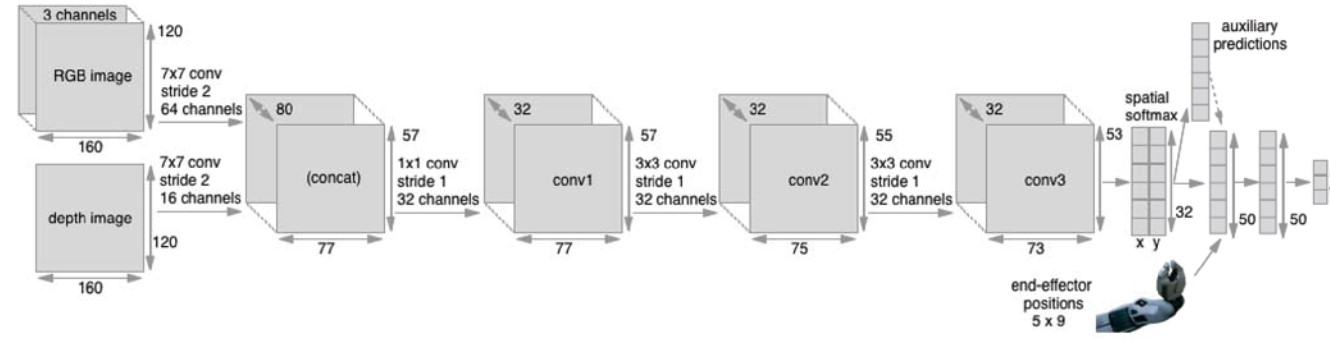
\includegraphics[width=0.9\textwidth]{figures/images/deep_imitation_bc/deep_imitation_bc.jpg}
    \caption{Architecture proposed in~\cite{zhang2018deep_vr_teleoperation}}
    \label{fig:deep_bc}
\end{figure}

% \usepackage{graphicx}
% \usepackage{hhline}


\begin{table}
    \centering
    \caption{Statistics of Training set, and Test Success rate~\cite{zhang2018deep_vr_teleoperation}}
    \label{table:deep_vr_teleoperation_results}
    \resizebox{\linewidth}{!}{%
    \begin{tabular}{|c|c|c|c|c|c|c|c|c|c|c|} 
    \hline
    \textbf{Task} & \textbf{Reaching} & \textbf{Grasping} & \textbf{Pushing} & \textbf{Plane} & \textbf{Cube} & \textbf{Nail} & \begin{tabular}[c]{@{}c@{}}\textbf{Grasp-}\\\textbf{and-}\\\textbf{Place}\end{tabular} & \begin{tabular}[c]{@{}c@{}}\textbf{Grasp-}\\\textbf{Drop-}\\\textbf{Push}\end{tabular} & \begin{tabular}[c]{@{}c@{}}\textbf{Grasp-}\\\textbf{Place-x2}\end{tabular} & \textbf{Cloth} \\ 
    \hhline{|===========|}
    \#demo & 200 & 180 & 175 & 319 & 206 & 215 & 109 & 100 & 60 & 100 \\ 
    \hline
    \begin{tabular}[c]{@{}c@{}}demo duration \\(min)\end{tabular} & 13.7 & 11.1 & 16.9 & 25.0 & 12.7 & 13.6 & 12.3 & 14.5 & 11.6 & 10.1 \\ 
    \hline
    \begin{tabular}[c]{@{}c@{}}Test success rate\\(\%)\end{tabular} & 91.6 & 97.2 & 98.9 & 87.5 & 85.7 & 87.5 & 96.0 & 83.3 & 80.0 & 97.4 \\
    \hline
    \end{tabular}
    }
    \end{table}
\paragraph*{Interactive Imitation Learning}\mbox{}\\
The Interactive Imitation Learning approach encompasses all methods specifically designed to address or mitigate the compounding-error phenomenon, which was first described in~\cite{pomerleau1988alvinn}.

As previously mentioned, this problem arises from the fact that, while Behavioral Cloning (BC) primarily follows a supervised learning procedure, it does not satisfy the i.i.d. assumption. This is because the agent's actions influence subsequent observations, creating a dependency between samples in the training set. As a result, when the agent interacts with the environment, even small errors can lead to new observations that fall outside the training distribution, potentially leading to an unrecoverable situation that the robot cannot resolve autonomously.

The significance of this problem was first formalized in \cite{ross2010efficient_reductions}. The authors observed that if a system makes an error with probability $\epsilon$ in a task with a time horizon of $T$, then, due to the compounding of errors, a supervised learner incurs a quadratic total cost of $O(\epsilon \ T^{2})$, instead of the expected linear cost of $O(\epsilon \ T)$. The quadratic term arises because, at any given time step $t$, the agent's state is influenced by errors made in the previous $t-1$ steps. This cumulative effect breaks the independence assumption typically held in the i.i.d. setting.

To attenuate this problem, interactive supervised learning algorithms have been proposed, such as the well-known \textit{DAgger} \cite{ross2011dagger}. Algorithm \ref{alg:dagger} describes the DAgger procedure. It is an aggregation strategy, based on the idea to train the policy $\pi^{L}$ under the state-distribution induced by the policy itself, but with the correct action performed by the expert. The main problem with DAgger is that it requires the expert to interact with the system during the training, introducing both \textbf{safety} and \textbf{data-efficiency} problems, especially when the system does not provide the human expert with sufficient control authority during the sampling process \cite{laskey2017comparing_hc_rc}. 
\begin{algorithm}
\caption{DAgger Algorithm \cite{ross2011dagger}}\label{alg:dagger}
\begin{algorithmic}
\Require Initial Dataset $\mathcal{D} \leftarrow \emptyset$, Initial policy $\pi^{L}_{1}$
\Ensure The best policy $\pi^{L}_{i}$
\For {$i=1, \dots N$}
    \State Sample $T-step$ trajectories using $\pi^{L}_{i}$
    \State Let $\mathcal{D}_{i} = {(s_{t}, \pi^{E}(s_{t}))}$, state $s_{t}$ visited by policy $\pi^{L}_{i}$, and actions given by the expert
    \State Aggregate Dataset, $\mathcal{D} \leftarrow \mathcal{D} \bigcup \mathcal{D}_{i}$
    \State Train policy $\pi^{L}_{i}$ on $\mathcal{D}$
    \State Let $\pi^{L}_{i+1} = \beta_{i}\pi^{E} + (1- \beta_{i})\pi^{L}_{i}$
\EndFor
\end{algorithmic}
\end{algorithm}

Human-Guided DAgger (HG-DAgger) \cite{kelly2019hg_dagger} is an enhancement of the traditional DAgger strategy, where a human expert oversees the rollout of the current policy. If the agent moves into an unsafe region of the state space, the expert steps in to guide the system back to safety. specifically, HG-DAgger was proposed in the context of autonomous vehicle driving, however, in \cite{jang2022bc_z}, it was shown that HG-DAgger is particularly effective in robotic manipulation tasks. The study found that, given the same total number of episodes, a policy trained exclusively on expert demonstrations has a significantly lower success rate than one trained on a dataset that includes both expert demonstrations and expert corrections.

In the context of Interactive Learning for Robot Manipulation, other works of interest include \cite{mandlekar2020human_in_the_loop,chisari2022correct}. 

In \cite{chisari2022correct}, a human expert provides both \textbf{corrective} and \textbf{evaluative} feedback. The former consists in the human that takes control of the robot to adjust the trajectory, the latter consists in a scalar weight $q$, set to 1 if the trajectory is satisfactory, 0 if the trajectory is not satisfactory, $\alpha$ if the trajectory is adjusted by the expert, where $\alpha$ is the ratio between non-corrected and corrected samples. Then a Neural Network was trained by minimizing a weighted version of the maximum-likelihood, $\mathcal{L}(a_{t},s_{t}) = - q \ log(\pi^{L}_{\theta}(a_{t}|s_{t}))$. Real-world experiments show that with a training time of \textbf{41 minutes}, including environmental reset, it was possible to have an agent capable of performing tasks such as picking up a cube or pulling a plug.



\paragraph*{Multi-Task Imitation Learning}\mbox{}\\
\textit{Multi-Task Imitation Learning} enables the learning and execution of multiple tasks from a set of demonstrations, highlighting the scalability and versatility of these methods.
\paragraph*{Object-Oriented Imitation Learning}\mbox{}\\
\textit{Object-Oriented Imitation Learning} focuses on learning behaviors in relation to specific objects and their interactions, providing a more structured and contextual approach to imitation learning.

\paragraph{Discussion}